\documentclass[10pt]{article}
\usepackage{tikz}
\usetikzlibrary{shapes.misc}
\usepackage[margin=0cm]{geometry}
\pagestyle{empty}
\tikzstyle{every node}=[cross out, draw, red]

\begin{document}

\vspace*{\fill}
\begin{center}
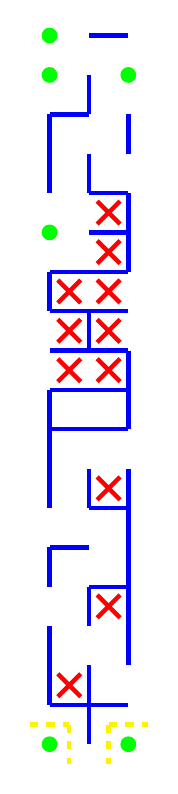
\begin{tikzpicture}[x=0.5cm, y=-0.5cm, ultra thick, blue]
% Walls
    \draw (1,0) -- (2,0);
    \draw (0,2) -- (1,2);
    \draw (1,4) -- (2,4);
    \draw (1,5) -- (2,5);
    \draw (0,6) -- (2,6);
    \draw (0,7) -- (2,7);
    \draw (0,8) -- (2,8);
    \draw (0,9) -- (2,9);
    \draw (0,10) -- (2,10);
    \draw (1,12) -- (2,12);
    \draw (0,13) -- (1,13);
    \draw (1,14) -- (2,14);
    \draw (0,17) -- (2,17);
    \draw (0,2) -- (0,4);
    \draw (0,6) -- (0,7);
    \draw (0,9) -- (0,12);
    \draw (0,13) -- (0,14);
    \draw (0,15) -- (0,17);
    \draw (1,1) -- (1,2);
    \draw (1,3) -- (1,4);
    \draw (1,7) -- (1,8);
    \draw (1,11) -- (1,12);
    \draw (1,14) -- (1,15);
    \draw (1,16) -- (1,18);
    \draw (2,2) -- (2,3);
    \draw (2,4) -- (2,6);
    \draw (2,8) -- (2,10);
    \draw (2,11) -- (2,16);
% Pillars
    \fill[green] (0,0) circle(0.2);
    \fill[green] (0,1) circle(0.2);
    \fill[green] (2,1) circle(0.2);
    \fill[green] (0,5) circle(0.2);
    \fill[green] (0,18) circle(0.2);
    \fill[green] (2,18) circle(0.2);
% Inner points in accessible cul-de-sacs
    \node at (1.5,4.5) {};
    \node at (1.5,5.5) {};
    \node at (0.5,6.5) {};
    \node at (1.5,6.5) {};
    \node at (0.5,7.5) {};
    \node at (1.5,7.5) {};
    \node at (0.5,8.5) {};
    \node at (1.5,8.5) {};
    \node at (1.5,11.5) {};
    \node at (1.5,14.5) {};
    \node at (0.5,16.5) {};
% Entry-exit paths without intersections
    \draw[dashed, yellow] (-0.5,17.5) -- (0.5,17.5);
    \draw[dashed, yellow] (1.5,17.5) -- (2.5,17.5);
    \draw[dashed, yellow] (0.5,17.5) -- (0.5,18.5);
    \draw[dashed, yellow] (1.5,17.5) -- (1.5,18.5);
\end{tikzpicture}
\end{center}
\vspace*{\fill}

\end{document}
